\documentclass{article}
\usepackage{amsmath}
\usepackage{graphicx}
\usepackage[utf8]{inputenc}
\usepackage{pgfplots}
\usepackage{hyperref}
\pgfplotsset{compat=1.18}

\title{BirdSynth: An ESP32 Digital Bird Synthesizer}
\author{}
\date{}

\begin{document}
\maketitle
\begin{figure}[h!]
    \centering
    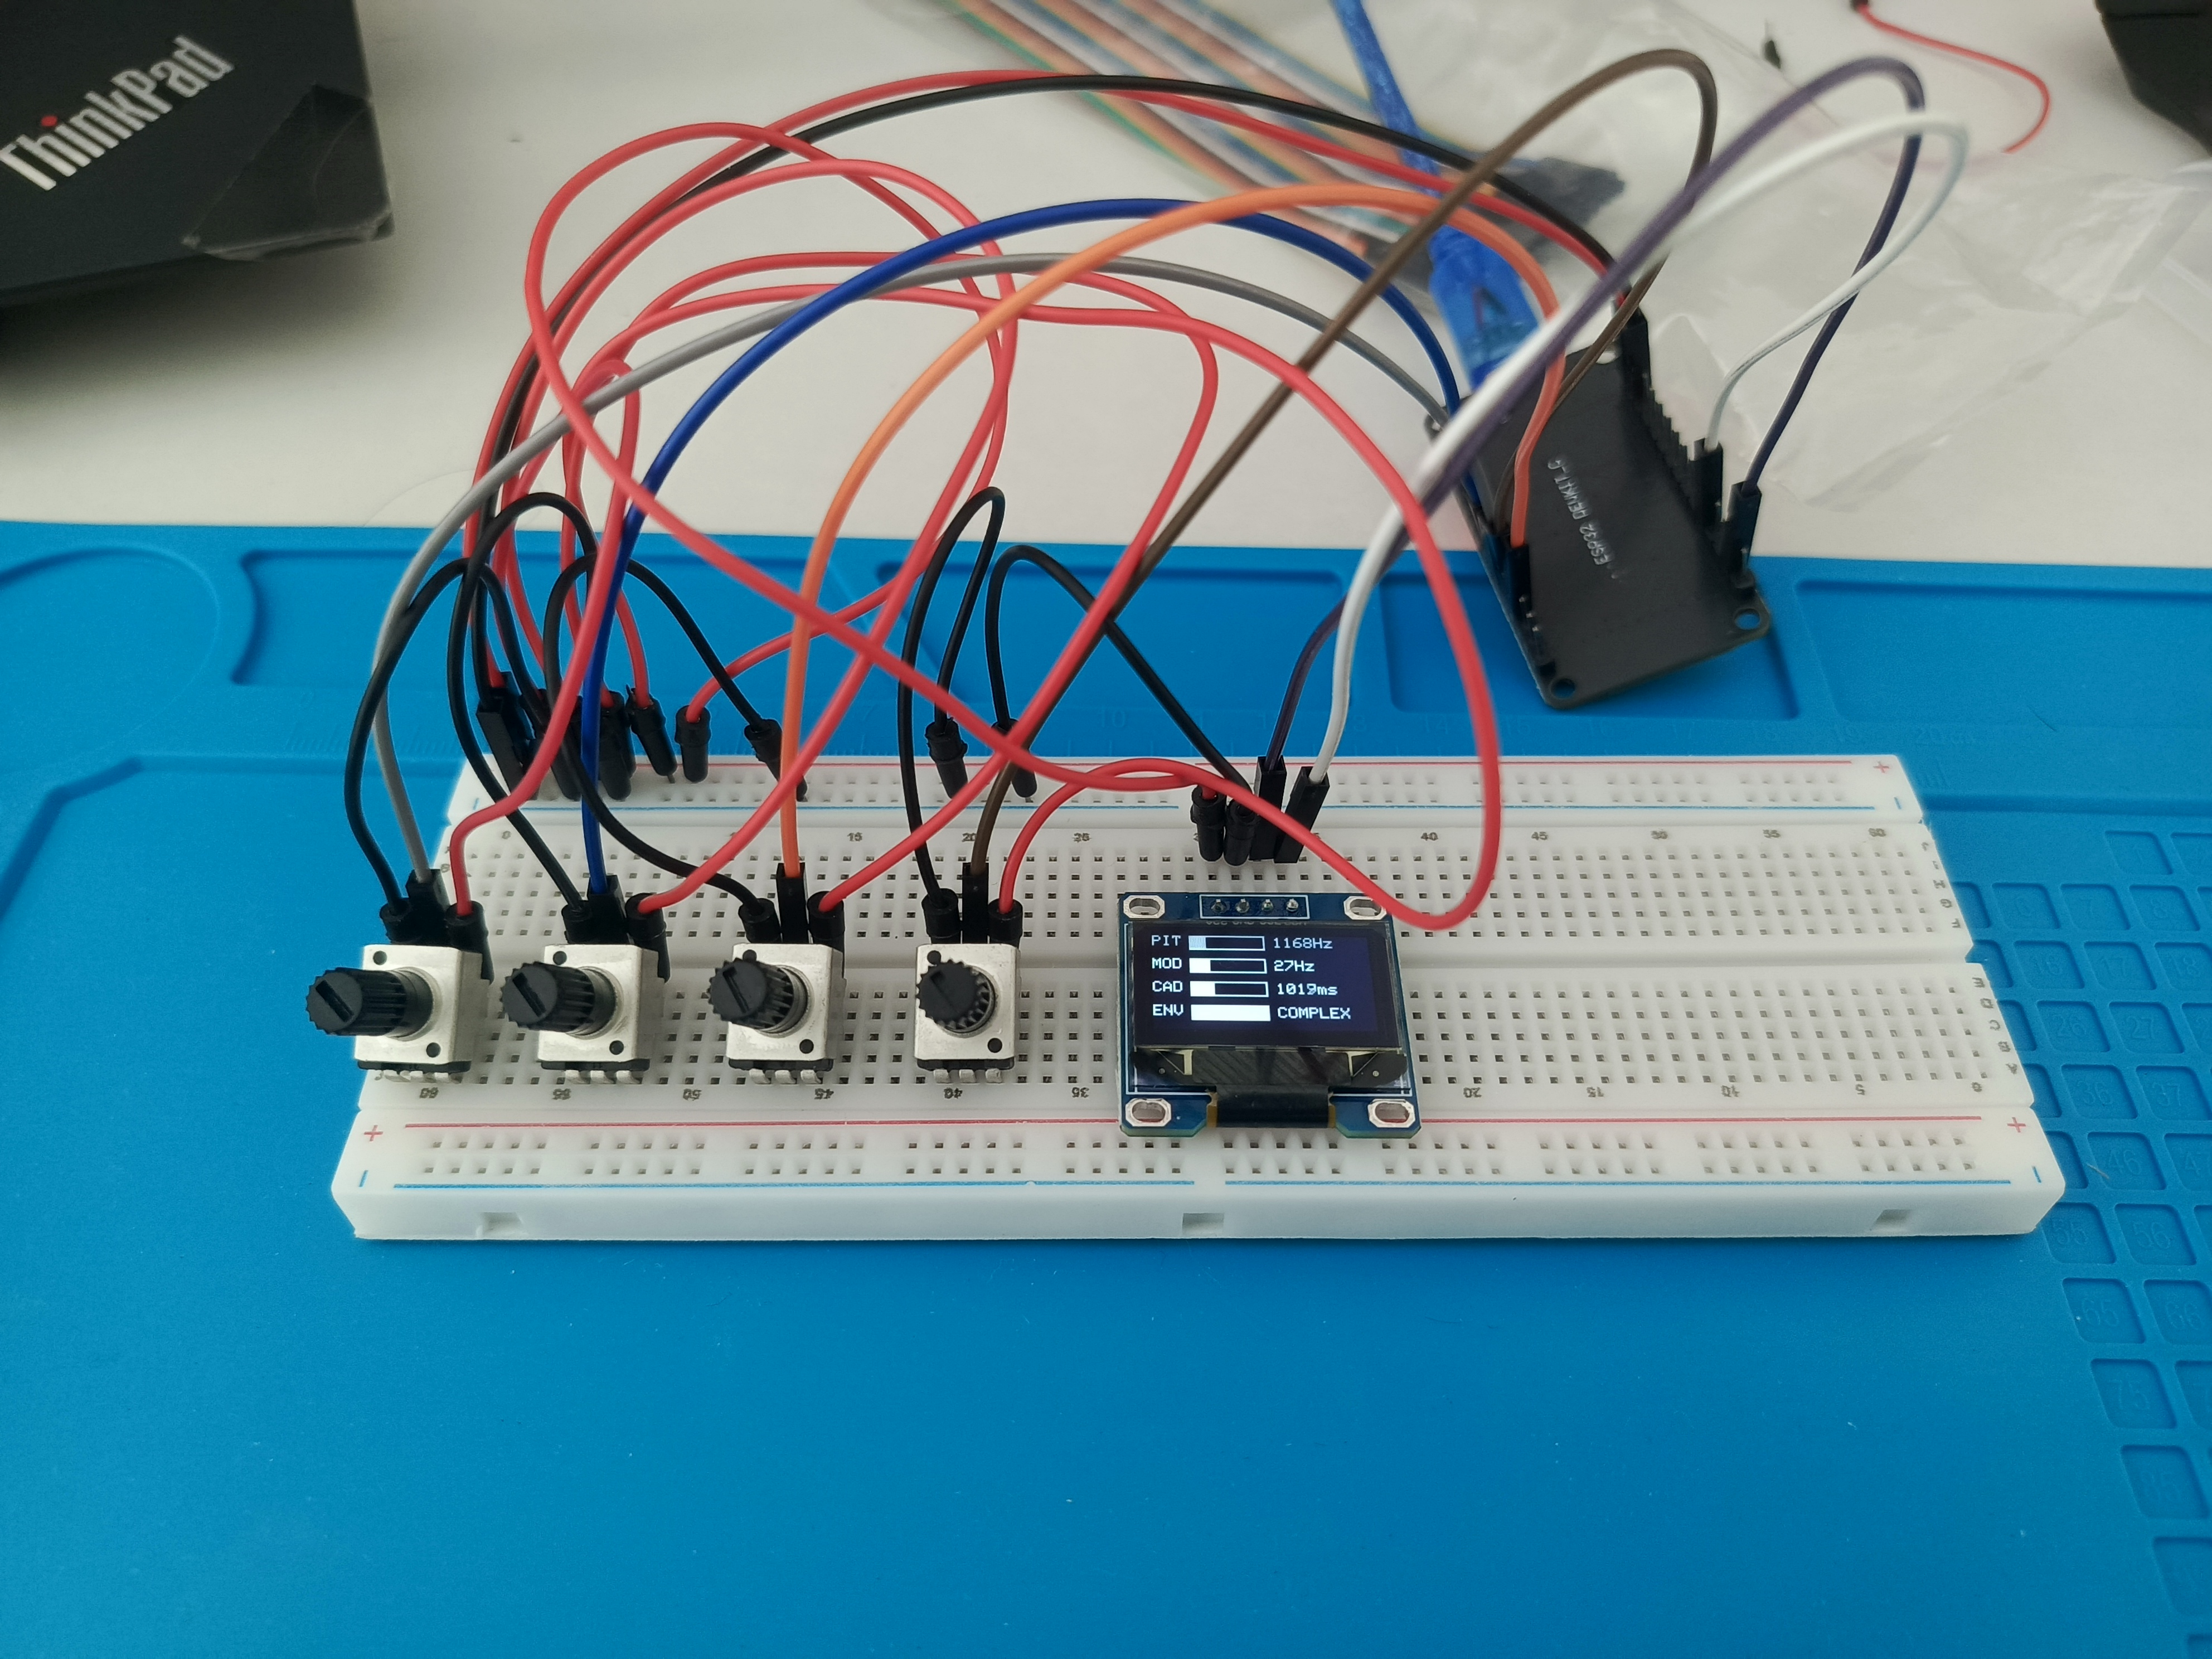
\includegraphics[width=1\linewidth]{On-board.jpg}
    \caption{Circuit of BirdSynth}
    \label{fig:placeholder}
\end{figure}

\section*{Background}
One time I visited a museum and there was an interesting exhibition showcasing different calls of a variety of birds. I found that very interesting and and want to try and build something similar. Although that exhibition used the recorded calls of the birds, I thought synthesizing them from basic elements would be a great idea and could be an interesting way for us to observe how certain variables interact and combine into the sounds that we hear coming out of the trees when we wake up in the morning (or stayed up to late). 

\section*{Hardware Components}
Here are the hardware that we used for the project:

\begin{itemize}
    \item \textbf{ESP32 Microcontroller}: This dual-core chip acts as the brain of the synthesizer. We split the workload: Core 0 handles the graphical interface and reads the physical knobs, while Core 1 is strictly dedicated to high-speed audio calculation and USB telemetry.
    \item \textbf{Potentiometers (Knobs)}: As shown on the breadboard, there are four potentiometers. These act as analog inputs, allowing for real-time control over the bird sound's parameters: Pitch, Modulation, Cadence, and Envelope. 
    \item \textbf{0.96-inch OLED Screen}: We use this as visual indicators for this project. It draws live progress bars for the 4 parameters so you can see exactly where the knobs are dialed in.
\end{itemize}

\noindent
For a setup with an external speaker we can use a DAC and amplifier like the GY-PCM5102 and the PAM8403.

\section*{The Math: Synthesis \& Variables}

We utilize the four variables to shape the bird sound synthesis and try to make it more organic sounding.

\subsection*{1. Pitch (Carrier Frequency, $f_c$)}
This is the foundational pitch of the bird chirp, mapped between 300Hz and 4000Hz. A lower knob value results in a slower wave (lower pitch), while a higher value creates a tighter, faster wave (higher pitch).

\begin{center}
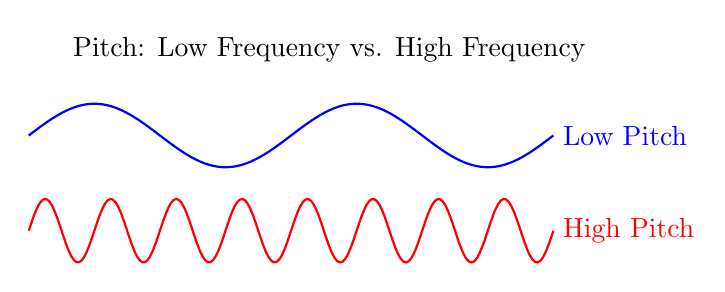
\begin{tikzpicture}
\begin{axis}[
    width=0.9\textwidth, height=4cm, 
    domain=0:4*pi, samples=200, 
    xmax=16, % Extended to make room for text
    axis lines=none, 
    title={Pitch: Low Frequency vs. High Frequency}
]
    % Low Pitch
    \addplot [blue, thick] {sin(deg(x)) + 2.5}; 
    \node[blue, right] at (axis cs: 4*pi, 2.5) {Low Pitch};
    
    % High Pitch
    \addplot [red, thick] {sin(deg(4*x)) - 0.5}; 
    \node[red, right] at (axis cs: 4*pi, -0.5) {High Pitch};
\end{axis}
\end{tikzpicture}
\end{center}

\subsection*{2. Modulation (Mod Freq, $f_m$, and Depth)}
This dictates how fast and how intensely the base pitch trills or wavers. To generate the sound digitally, the ESP32 calculates the phase increments for the modulator wave:
$$ \text{inc}_m = \frac{2\pi \cdot f_m}{\text{sampleRate}} $$

It then generates the modulation wave and multiplies it by the modulation depth (scaled to 40\% of the carrier frequency):
$$ \text{$mod_{wave}$} = \sin(\text{phase}_m) \times \text{modDepth} $$

This modulation wave offsets the base pitch, creating the final, fluctuating frequency for the current audio sample:
$$ f_{\text{current}} = f_c + \text{mod\_wave} $$

\begin{center}
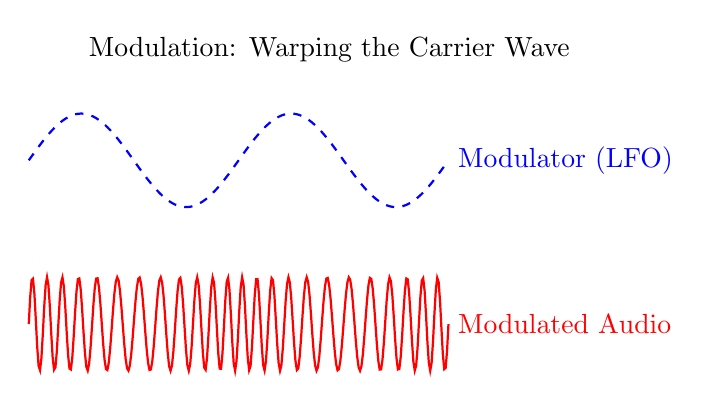
\begin{tikzpicture}
\begin{axis}[
    width=0.9\textwidth, height=5.5cm, 
    domain=0:4*pi, samples=300, 
    xmax=20, % Extended to make room for long text labels
    axis lines=none, 
    title={Modulation: Warping the Carrier Wave}
]
    % Modulator Wave 
    \addplot [blue, thick, dashed] {sin(deg(x)) + 2.5};
    \node[blue, right] at (axis cs: 4*pi, 2.5) {Modulator (LFO)};
    
    % FM Wave 
    \addplot [red, thick] {sin(deg(12*x + 2.5*sin(deg(x)))) - 1};
    \node[red, right] at (axis cs: 4*pi, -1) {Modulated Audio};
\end{axis}
\end{tikzpicture}
\end{center}

\subsection*{3. Cadence}
Cadence controls the timing and delay between the chirps. Instead of a continuous drone, birds chirp in bursts. This variable dictates the pauses, ranging from rapid-fire 100ms bursts to longer 3000ms pauses.

\begin{center}
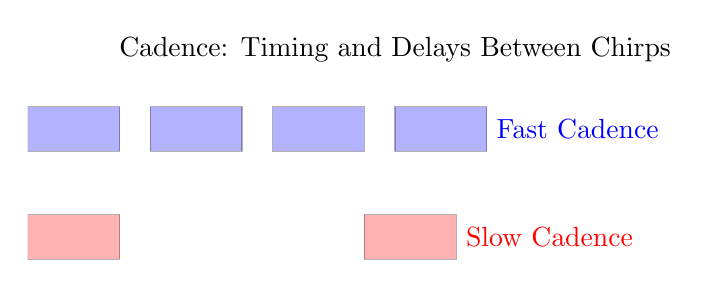
\begin{tikzpicture}
\begin{axis}[
    width=0.9\textwidth, height=4cm, 
    xmin=0, xmax=12, ymin=-1.5, ymax=1.5, % Extended xmax for labels
    axis lines=none, 
    title={Cadence: Timing and Delays Between Chirps}
]
    % Fast Cadence
    \draw[fill=blue, opacity=0.3] (0, 0.5) rectangle (1.5, 1.2);
    \draw[fill=blue, opacity=0.3] (2, 0.5) rectangle (3.5, 1.2);
    \draw[fill=blue, opacity=0.3] (4, 0.5) rectangle (5.5, 1.2);
    \draw[fill=blue, opacity=0.3] (6, 0.5) rectangle (7.5, 1.2);
    \node[blue, right] at (7.5, 0.85) {Fast Cadence};

    % Slow Cadence
    \draw[fill=red, opacity=0.3] (0, -1.2) rectangle (1.5, -0.5);
    \draw[fill=red, opacity=0.3] (5.5, -1.2) rectangle (7.0, -0.5);
    \node[red, right] at (7.0, -0.85) {Slow Cadence};
\end{axis}
\end{tikzpicture}
\end{center}

\subsection*{4. Envelope (ENV)}
While the carrier and modulator define the frequencies, the envelope dictates the overall volume shape (Attack and Decay) of the synthesized sound over time, giving it a natural, plucked, or swelling characteristic rather than a harsh beep.

\begin{center}
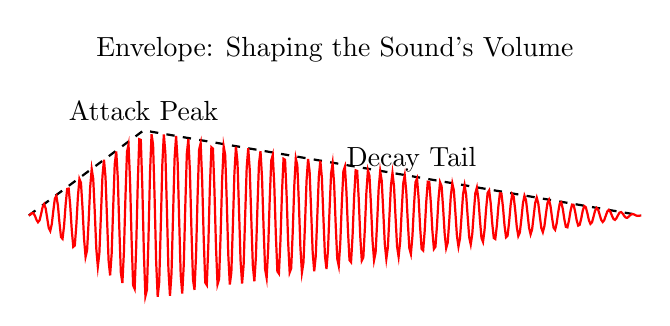
\begin{tikzpicture}
\begin{axis}[
    width=0.9\textwidth, height=4.5cm, 
    domain=0:8, samples=400, 
    ymax=1.5, % Extended ymax so the top label doesn't get cut off
    axis lines=none, 
    title={Envelope: Shaping the Sound's Volume}
]
    % Envelope Outline (Dashed)
    \addplot [black, thick, dashed] coordinates {(0,0) (1.5,1) (8,0)};
    \node[black, above] at (1.5, 1) {Attack Peak};
    \node[black, above] at (5, 0.4) {Decay Tail};
    
    % Filled/shaped wave
    \addplot [red, thick] { (x<=1.5)*(x/1.5)*sin(deg(40*x)) + (x>1.5)*(1 - (x-1.5)/6.5)*sin(deg(40*x)) };
\end{axis}
\end{tikzpicture}
\end{center}

\section*{Digital Recording via Python}
To more accuractely capture audio we stream the pure digital audio telemetry directly to a computer. 

\begin{itemize}
    \item The ESP32 sends 16-bit audio data over serial at an ultra-fast baud rate of 921600.
    \item A custom Python script opens this serial port and constantly listens for a specific text packet starting with ``SYNC:''. When detected, it parses the live knob data (Pitch, Mod, Cadence, Env) and prints it neatly to the terminal.
    \item Immediately following the text, the script grabs the raw binary audio data in 512-byte chunks.
    \item It uses the \texttt{pyaudio} library to stream the sound to the computer's speakers in real time.
    \item Concurrently, it uses Python's native \texttt{wave} library to write these raw frames directly into a \texttt{.wav} file.  
\end{itemize}

\section*{Demo}
Here are some demonstration of our Bird Synthesizer mimicing popular birds
\subsection*{Great Horned Owl}
\href{https://youtu.be/du914pfOyX8}{Video}.
\subsection*{American Crow}
\href{https://youtu.be/UnQx-fNgLME}{Video}.
\subsection*{Red Tailed Hawk}
\href{https://youtu.be/X9xNjkKIluQ}{Video}.
\subsection*{Can you guess this one}
\href{https://youtu.be/KUNCZCRVAMI}{Video}.
\end{document}